\documentclass[tikz,border=6pt]{standalone}
% Shared style for the HERMESS schematic figures (compiled by build.sh).
% ETH palette; Latin Modern (the LaTeX default) to match the documentation.
\usepackage{amsmath}
\usepackage{tikz}
\usetikzlibrary{arrows.meta,positioning,calc,shapes.geometric,circuits.ee.IEC}
\definecolor{ethblue}{HTML}{215CAF}
\definecolor{ethpetrol}{HTML}{007894}
\definecolor{ethgrey}{HTML}{6F6F6F}
\tikzset{
  block/.style      = {draw=ethblue, thick, fill=ethblue!8, minimum height=9mm,
                       minimum width=16mm, inner sep=2.5pt, align=center},
  sum/.style        = {draw=ethblue, thick, circle, fill=white, minimum size=4.5mm, inner sep=0pt},
  sig/.style        = {-{Latex[length=2.4mm]}, thick},
  wire/.style       = {thick},
  node distance     = 9mm and 12mm,
  every node/.style = {font=\small},
  lbl/.style        = {font=\small, inner sep=1.5pt},
  port/.style       = {font=\small\itshape, text=ethgrey},
}

\begin{document}
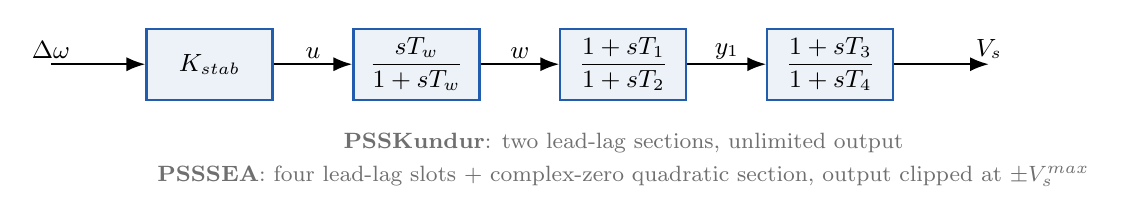
\begin{tikzpicture}
  \node[block] (gain) {$K_{stab}$};
  \node[block, right=10mm of gain] (wo) {$\dfrac{sT_w}{1 + sT_w}$};
  \node[block, right=10mm of wo] (ll1) {$\dfrac{1 + sT_1}{1 + sT_2}$};
  \node[block, right=10mm of ll1] (ll2) {$\dfrac{1 + sT_3}{1 + sT_4}$};
  \draw[sig] ($(gain.west)+(-1.2,0)$) node[above, lbl] {$\Delta\omega$} -- (gain);
  \draw[sig] (gain) -- (wo) node[midway, above, lbl] {$u$};
  \draw[sig] (wo) -- (ll1) node[midway, above, lbl] {$w$};
  \draw[sig] (ll1) -- (ll2) node[midway, above, lbl] {$y_1$};
  \draw[sig] (ll2.east) -- ++(1.2,0) node[above, lbl] {$V_s$};
  \node[lbl, text=ethgrey, align=center] at ($(ll1.south)+(0.0,-0.75)$)
    {\footnotesize \textbf{PSSKundur}: two lead-lag sections, unlimited output\\[1pt]
     \footnotesize \textbf{PSSSEA}: four lead-lag slots + complex-zero quadratic section, output clipped at $\pm V_s^{max}$};
\end{tikzpicture}
\end{document}
